\documentclass{report}
\usepackage[T1]{fontenc} % Fontes T1
\usepackage[utf8]{inputenc} % Input UTF8
\usepackage[backend=biber, style=ieee]{biblatex} % para usar bibliografia
\usepackage{csquotes}
\usepackage[portuguese]{babel} %Usar língua portuguesa
\usepackage{blindtext} % Gerar texto automaticamente
\usepackage[printonlyused]{acronym}
\usepackage{hyperref} % para autoref
\usepackage{graphicx}
\usepackage[backend=biber]{biblatex}
\bibliography{bibliografia}


\begin{document}

%   Definições    %

\def\titulo{TERRORISMO}
\def\subtitulo {CIBERTERRORISMO}
\def\data{2017-2018}
\def\autores{Márcia Pires, Rita Amante}
\def\autorescontactos{(88747) marcia.pires@ua.pt, (89264) rita.amante@ua.pt}
\def\versao{VERSÃO 1}
\def\departamento{Departamento de Eletrónica, Telecomunicações e Informática}
\def\empresa{Universidade de Aveiro }
\def\logotipo{ua.pdf}


% CAPA %

\begin{titlepage}

\begin{center}

\vspace*{50mm}
{\Huge \textbf{\titulo}}\\ 
\vspace{10mm}
{\Large\textbf{\subtitulo}}\\
\vspace{10mm}
{\Large \empresa}\\
\vspace{10mm}
{\LARGE \autores}\\ 
\vspace{30mm}

\begin{figure}[h]
\center
\includegraphics{\logotipo}
\end{figure}
\vspace{20mm}
\end{center}

\begin{flushright}
\versao
\end{flushright}
\end{titlepage}

% Página de Título %
\title{
{\Huge\textbf{\titulo}}\\
\vspace{2.5mm}
{\Large\textbf{\subtitulo}}\\
\vspace{10mm}
{\large \departamento\\ \empresa}
}
\vspace{05mm}
\author{
\vspace{2.5mm}
    \autores \\
    \autorescontactos
}
\vspace{05mm}
\date{\data}
\maketitle
\pagenumbering{roman}

%%%%%% RESUMO %%%%%%
\begin{abstract}
\paragraph{} Vivemos num mundo cada vez mais perigoso e hostil, onde somos constantemente testemunhas das atrocidades terroristas que atualmente ameaçam todos os países e indivíduos.\par 
Nos dias de hoje, os atos terroristas têm sido banalizados dada a frequência da sua ocorrência, provocando um sentimento de insegurança e medo nos cidadãos do mundo. E esse sentimento é ainda mais acentuado quando, ao olharmos para a realidade atual do mundo em que vivemos, nos damos conta que, se no passado todos os ataques eram físicos e havia fronteiras delimitadores dos Estados. Hoje assiste-se a uma globalização do mundo e podemos ser igualmente atacados no mundo virtual. Tudo isto porque as relações sociais entre os indivíduos estão combinadas em espaços reais e virtuais de comunicação e, portanto, a vida é, neste momento, impensável sem o uso da Internet. Ora a dependência deste uso torna-nos cada vez mais vulneráveis e suscetíveis aos ataques cibernautas. Deste modo, é previsível que os terroristas, com o decorrer dos anos, comecem cada vez mais a substituir os métodos tradicionais do terrorismo por métodos virtuais, dada a facilidade e também acessibilidade a conteúdos anteriormente inacessíveis. É, desta forma, instaurada uma nova preocupação no quotidiano que se aproxima, e a dúvida acerca do sucesso deste novo terrorismo.
\end{abstract}

% Agradecimentos %
% Segundo glisc deveria aparecer após conclusão...
\renewcommand{\abstractname}{Agradecimentos}
\begin{abstract}
\paragraph{} Ao Professor António Adrego Rocha pelo apoio prestado e paciência que teve ao ensinar-nos a trabalhar com este programa, orientando-nos sempre que necessário.
\paragraph{} Ao Professor Rui Quintela que durante o 12º ano nos incentivou a trabalhar com computadores, nas aulas de Aplicações Informáticas.
\paragraph{} Aos nossos Pais, familiares e amigos, que sempre nos apoiaram e encorajam nas horas mais difíceis.
\paragraph{} Por fim, a todos os nossos Professores do passado e do presente, por todo o conhecimento que verteram em nós e que se têm mostrado útil nas mais diversas ocasiões.
\end{abstract}

%%%%%%%%%%%%%%%%%%%%%%%%%%%%%%%
\tableofcontents
% \listoftables     % descomentar se necessário
% \listoffigures    % descomentar se necessário

\clearpage
\pagenumbering{arabic}
%%%%%%%%%%%%%%%%%%%%%%%%%%%%%%%%


% Introdução %

\chapter{Introdução}
\label{chap.introducao}

\paragraph{} Os temas abordados neste trabalho são o terrorismo e o ciberterrorismo. De forma a ajudar a sua exposição, dividiu-se o documento em dezasseis capítulos.\par
Os primeiros dez capítulos são referentes ao tema terrorismo, onde é apresentada uma passível definição, o surgimento histórico, os tipos, causas e consequências do terrorismo, e ainda, grupos e ataques terroristas.\par
Do capítulo décimo primeiro ao décimo quarto, o tema abordado é o ciberterrorismo, onde é apresentada a sua definição, formas, níveis e exemplos de atos de ciberterrorismo.\par
A finalizar, no capítulo décimo quinto, são apresentadas as conclusões do trabalho.


% Capítulo 2 - Definição de Terrorismo %

\chapter{Definição de Terrorismo}
\label{chap.Definição de Terrorismo}

\paragraph{} O terrorismo é um fenómeno social complexo e multifacetado, tanto no âmbito das causas como dos efeitos, de grande impacto na paz e na segurança internacional, que influencia as relações entre os Estados e as Comunidades.\par
A definição de terrorismo está relacionada com a história, a cultura e as políticas das nações e organizações internacionais.\par
O terrorismo pode ser interpretado como um crime, como um ato de guerra, como um ato religioso ou como um ato político. Cabe salientar que não existe uma abordagem certa ou errada, e elas não são excludentes entre si. É inegável que se trata de um ato, prática e método criminoso injustificável, onde quer que seja cometido e por quem o cometa/apoie, direita ou indiretamente, que põe em risco a vida de inocentes, põe em causa liberdades fundamentais e a dignidade dos seres humanos.\par
A Organização das Nações Unidas (ONU), define terrorismo como:
\begin {quotation}
"Atos criminosos pretendidos ou calculados para provocar um estado de terror no público em geral […]."
\end {quotation}
\par
Todas as definições de terrorismo estão carregadas de juízos de valor e isto é particularmente verdadeiro quando analisadas todas as tentativas de definição no sentido de clarificar a natureza jurídica do terrorismo. Deste modo, não existe ainda uma formulação geralmente reconhecida daquilo que se pode considerar em termos genéricos como um ato terrorista. \par  
O terrorismo é descrito como uma tática e estratégia, como um crime e um dever sagrado.  Este depende muito do ponto de vista em que é analisado. 

% Capítulo 3 - Surgimento Histórico do Terrorismo %

\chapter{Surgimento Histórico do Terrorismo}
\label{chap.Surgimento Histórico do Terrorismo}

\paragraph{} A primeira organização conhecida que exibiu semelhanças com as organizações terroristas atuais era composta pelos Fanáticos da Judeia. Apelidados pelos Romanos de Sicarii, eles organizavam campanhas de assassinatos aos Romanos e a todos os judeus que tinham colaborado com eles. Os seus motivos derivavam de uma crença intransigente de que os Romanos não se podiam manter fiéis às ditaduras judaicas enquanto vivessem como sujeitos Romanos. Eventualmente, a revolta dos Fanáticos tornou-se conhecida e eles finalmente assediaram e cometeram suicídios em massa na fortificação de Masada.\par
A Revolução Francesa promoveu o primeiro uso das palavras "Terrorista"\, e "Terrorismo". O uso da palavra "terrorismo"\, começou no ano de 1795, referindo-se ao "Reinado do Terror"\, iniciado pelo governo revolucionário. Os agentes da Comissão de Defesa Pública e da Convenção Nacional que aplicaram as políticas "d`O Terror" \, foram mencionados como "Terroristas". A Revolução Francesa providenciou um exemplo a futuro estados, oprimindo as suas populações, o que inspirou a reação de realistas e outros oponentes da Revolução que empregaram práticas terroristas tais como o "assassinato" \, e a "intimidação" \, em resistência a para os agentes Revolucionários. A máfia Parisiense teve um papel crítico em momentos chave antes, durante e depois da Revolução. Tais atividades ilegais como a morte de oficiais e aristocratas em espetáculos horríveis começaram muito antes da primeira utilização da guilhotina.\par
Perante o exposto, podemos dizer que o terrorismo não tem um momento preciso de surgimento histórico. No entanto, podemos considerar que o terrorismo surgiu com o Estado e com a implementação de políticas injustas para com a população. 


% Cap 4 - Porque surgiu o Terrorismo? %

\chapter{Porque surgiu o Terrorismo?}
\label{chap.Porque surgiu o Terrorismo?}

\paragraph{} Segundo David J. Whittaker, em 2003: 
\begin {quotation}
"Existem pré condições que a longo prazo podem incentivar um ato insurgente, assim como a falta de liberdade política, problemas sociais, problemas económicos, insegurança pública,... bem como precipitantes, que são eventos específicos que precedem um ato terrorista, tais como repressões policiais, eventos desportivos, eleições, etc."
\end {quotation}
\par
A maior parte dos atos terroristas são consequência de conflitos de larga duração. Em muitos desses conflitos, a violência gera violência. Assim, o terrorismo não é a causa dos conflitos, mas sim a sua expressão mais visível. Cresce onde existe instabilidade, divisão étnica e religiosa, violência e repressão.\par
Por vezes, em muitos lugares, unirmo-nos a um grupo extremista pode ser rentável; noutros, pode ser a única via para escapar à fome e à pobreza. \par
O fenómeno do terrorismo é extremamente complexo, visto que não há nenhuma causa única que explique por sí só este fenómeno. Há terroristas de várias classes (baixa, média, média-alta e rica), podendo-se dizer que não é um problema de falta de formação. Sem dúvida, os problemas sociais, de integração ou desenvolvimento da própria identidade, potenciam o fenómeno porque reunem pessoas vulneráveis que entram nessas correntes ideológicas do terrorismo.


% Capítulo 5 - Terrorismo vs Criminoso comum %

\chapter{Terrorismo vs Criminoso Comum}
\label{chap.Terrorismo vs Criminoso Comum}

\paragraph{} São várias as diferenças que encontramos entre terrorista e criminoso comum.\par
O terrorista tem objetivo político, motivação ideológica ou religiosa, foca-se no grupo, tem um propósito, é treinado para uma missão, é orientado para atacar e não tem sentido de auto preservação.\par
O criminoso comum, foca-se em si mesmo, num crime de oportunidade, sem filosofia ou doutrina, sem causa, sem treinamento, orientado para escapar e tem sentido de auto preservação.


% Capítulo 6 - Tipos de Terrorismo %

\chapter{Tipos de Terrorismo}
\label{chap.Tipos de Terrorismo}

\paragraph{} O terrorismo tem várias vertentes, podendo assim ser dividido em duas categorias:
\begin{itemize}
 \item Terrorismo Indiscriminado ou Aleatório;
 \item Terrorismo Seletivo. 
\end{itemize}

O \textbf{terrorismo indiscriminado ou aleatório} são todas as ações que se destinam a fazer um dano a um agente indefinido ou irrelevante. Como o próprio nome indica, impede-nos de definir antecipadamente a sua vítima e não obedece a qualquer seleção sistemática ou política. \par
Este tipo de terrorismo procura deliberada e indiscriminadamente fazer vítimas inocentes, em grande escala e com a maior diferença social possível. Assim, a universalidade da vítima é a principal caraterística deste terrorismo, tendo como objetivo criar um terror incontrolável e generalizado, e sendo aleatório, faz de todo o mundo um suspeito, tornando a sua repressão muito difícil. \par
A colocação de bombas em cafés, parques de estacionamento, entre outros, são alguns exemplos deste tipo de terrorismo. \par 
Por outro lado, temos o \textbf{terrorismo seletivo} que é caraterizado como um ato que visa um alvo reduzido, estudado e conhecido antes de ser efetuado. É alimentado através de chantagem, vingança e eliminação de um obstáculo. \par
Devido ao carácter seletivo é-nos permitido distinguir alguns tipos de terrorismo mais comuns, tais como:
\begin{itemize}
 \item Religioso;
 \item Nacionalista;
 \item Estado; 
 \item Bioterrorismo.
\end{itemize}

O \underline {terrorismo Religioso} está associado ao fundamentalismo e extremismo de membros de diferentes religiões que agem violentamente pelo facto de se definirem pela sua religiosidade (como ideologia ou etnia) sendo a religião preponderante nos objetivos e maneira de atuar do grupo. \par
O \underline {terrorismo Nacionalista} é realizado por grupos com fortes  ideologias nacionalistas, que desejam estabelecer um estado independente, tomar o controle da nação, ou derrubar um sistema político. \par
O \underline{terrorismo de Estado} surge quando os governos se impõem, de forma violenta, contra a sua sociedade ou um grupo de pessoas dominado, em que o grupo político que detém o poder utiliza o terror como instrumento de governabilidade. Consiste em desprezar uma sociedade, submetê-la a leis injustas, conduzi-la à angústia e empurrá-la à passagem definitiva do desespero. O Nazismo na Alemanha, o Estalinismo na União das Repúblicas Socialistas Soviéticas (URSS) e os regimes militares latino americanos são exemplos deste tipo de terrorismo. \par
O \underline {terrorismo Comunal ou Comunitário} são conflitos desordenados, que a população civil ou as suas autoridades intervêm diretamente, contra outras comunidades, geralmente minorias étnicas ou religiosas. Trata‐se de uma espécie de "terror coletivo", visando a expulsão ou eliminação destas. Este tipo de terrorismo tem vindo a crescer no Afeganistão, Paquistão e Índia e é o que produz o maior número de vítimas e destruições, como por exemplo, a Guerra Civil. \par
O \underline{Bioterrorismo} consiste em ataques em que ocorre uma libertação de vírus, bactérias ou outros agentes infeciosos, sendo talvez o tipo de terrorismo mais mortífero que existe. Exemplos deste tipo de terrorismo são a disseminação intencional de antraz ou a libertação do vírus da varíola, entre outros.


% Capítulo 7 - Causas/Motivações de Terrorismo %

\chapter{Causas do Terrorismo}
\label{chap.Causas do Terrorismo}

\paragraph{} O terrorismo pode ser visto como uma consequência das injustiças deste mundo que o fazem germinar nos meios mais pobres onde o desespero fomenta a vingança contra os poderosos. Assim, o sistema capitalista, segregador, elitista que visa apenas a promoção dos mais ricos sobre os mais pobres é um fator desencadeador que leva a ações terroristas. \par
A pobreza e as más condições económicas levam ao descontentamento, que gera sentimentos de revolta por falta de meios, o que leva à violência. \par
A não aceitação das diferenças comparativamente aos outros gera a opressão, a revolta e a violência.\par
O fanatismo religioso sempre foi um dos principais motivos para a morte de milhões de pessoas durante toda a história da humanidade. Muitas pessoas não percebem que para uma boa convivência não precisamos de acreditar e aceitar todos na mesma doutrina. O intercâmbio entre culturas e crenças é o que faz uma sociedade evoluir, ser dinâmica. Mas ao longo dos anos, muitas organizações religiosas tentaram forçar o contrário, criando doutrinas dogmáticas. As crenças levadas ao extremo, orgulho excessivo ou acontecimentos traumáticos, que levam ao descontentamento geram violência. \par
As ações militares fazem com que uma população/grupo alimente um sentimento de injustiça, o que traz ações violentas.\par
Quando a vida só oferece dor e sofrimento, e uma pessoa já não vê sentido nela, o desespero pode levar a um sentimento de vingança e morte. Normalmente a causa para este desespero é a desigualdade económica, social, étnica, entre outros, que atualmente se vive todos os dias, pois um mundo injusto torna-se um mundo inseguro.\par
No meio de uma guerra, uma parte da população que se vê sem meios para entrar diretamente nela tenta atingir as forças opressoras com pequenos ataques terroristas.\par
O racismo é um tema muito falado atualmente. O lema \textit {todos diferentes, todos iguais} não é ainda mundialmente aceite. Muitas pessoas consideram pessoas de outras etnias inferiores, achando que não deviam partilhar os mesmos direitos e deveres.\par
Assim podemos dizer, que as causas do terrorismo são diversas, destacando-se entre elas:
\begin{itemize}
 \item a pobreza;
 \item a discriminação/racismo;
 \item as guerras;
 \item o fanatismo;
 \item o desespero;
 \item a xenofobia. 
\end{itemize}

As causas do terrorismo podem variar consoante os interesses de cada região do mundo. A seguir, são apresentadas algumas das causas do terrorismo no Médio Oriente, na Europa e na América Latina.\par
As causas do \underline{terrorismo no Médio Oriente} são principalmente políticas. A disputa é pela posse da terra. Os palestinos consideram que o território ocupado por Israel lhes pertence por  direito. Além disso, Israel é o único país muçulmano, no Médio Oriente, logo claramente se destaca por ser "diferente" ou "invasor".\par
As causas do \underline{terrorismo Europeu} são principalmente económicas e idealistas. Movimentos extremistas pensam que a violência é necessária para derrubar o capitalismo.\par
As causas do \underline{terrorismo da América Latina} são essencialmente um produto de conflito entre classes. Até há pouco tempo, quase todas as nações da América Latina foram controladas por regimes corruptos e autoritários, vivendo a maioria das pessoas na pobreza. A força impulsionadora deste terrorismo é o desejo  de reorganizar a sociedade, retirar os interesses das empresas estrangeiras e redistribuir a terra e a riqueza. 


% Capítulo 8 - Consequências do Terrorismo %

\chapter{Consequências do Terrorismo}
\label{chap.Consequências do Terrorismo}

\paragraph{} Um ato terrorista traz consequências tanto a nível da integridade física como a nível psicológico.\par
A nível da integridade física, pode-se manifestar em graves ferimentos, mutilação de membros, incapacidade permanente, profunda alteração da saúde,  morte, entre outros.\par
A nível psicológico, as vítimas podem vir a sofrer de Perturbação Pós-Stress Traumático (PPTS), apresentando sintomas como: reviver o acontecimento, vezes sem conta; pensamentos indesejados, intrusivos e repetitivos; entorpecimento emocional; depressão; aumento do consumo de ansiolíticos; entre outros.\par
A nível emocional, provoca sentimento de perda, de luto pelos entes queridos, familiares ou amigos.\par
As consequências a nível económico/social têm sido demonstradas pela ampla perda material e financeira, tendo muitas das vítimas visto alteradas as suas fontes de rendimento, acabando por abdicar do seu trabalho devido a incapacidades parciais ou permanentes, ou mesmo, mudança de residência.\par
Podemos dizer que o primeiro efeito imediato que a população sofre é o pânico. A longo prazo, é o medo que acaba por triunfar sobre as vítimas. \par
Um ato de terror subtrai de suas vítimas a noção que elas tinham de paz, a sensação de segurança e independência.\par
Assim, são várias as consequências que podem surgir após um ato terrorista, a saber:
\begin{itemize}
 \item terror;
 \item trauma;
 \item desentendimento social;
 \item aumento da xenofobia contra a etnia ou nacionalidade dos terroristas;
 \item destruição;
 \item morte;
 \item prejuízos;
 \item quebra de confiança;
 \item isolamento/ solidão;
 \item dificuldade nas relações pessoais;
 \item silêncio;
 \item aumento da insegurança;
 \item instabilidade psicológica e económica.
\end{itemize}

% Capítulo 9 - Grupos Terroristas %
\chapter{Grupos Terroristas}
\label{chap.Grupos Terroristas}
\paragraph{} Há imensos grupos terroristas a nível mundial, motivados pelas mais diversas razões. Aqui, apresentamos apenas alguns dos grupos mais conhecidos.\par

\begin{itemize}
 \item \textbf{Al-Qaeda}
\end{itemize}
\par
Criada por Osama Bin Laden, em 1989, a Al-Qaeda  é uma organização terrorista formada, principalmente, por fundamentalistas islâmicos e árabes. Inicialmente o seu foco de atuação tinha por objetivo expulsar as tropas russas do território do Afeganistão.\par
Atualmente, a Al-Qaeda possui bases em vários países (Somália, Argélia, Líbia, Chade, etc.), suas ações terroristas ocorrem em nações ocidentais e em países muçulmanos que apoiam os Estados Unidos, como, a Arábia Saudita, a Turquia e a Indonésia.\par
Este grupo foi o responsável pelo atentado ao World Trade Center, Torres Gémeas e Pentágono, nos EUA a 11 de setembro de 2001.

\begin{itemize}
 \item \textbf{ETA}
\end{itemize}
\par
ETA ou Pátria Basca e Liberdade, foi fundado em 31 de julho de 1959 por estudantes nacionalistas que se rebelaram contra o "imobilismo" \, do Partido Nacionalista Basco (PNV) ante ao franquismo.\par
Grupo da região do País Basco que luta por uma independência política e territorial.\par
O atentado a nove de junho de 1987, onde um carro bomba explode no parque do centro  comercial Hipercor, em Barcelona, foi da responsabilidade deste grupo.

\begin{itemize}
 \item \textbf{IRA}
\end{itemize}
\par
Grupo terrorista irlandês católico, fundado em 1914, que pretendia separar a Irlanda do Norte do Reino Unido e vincular-se à República da Irlanda. Para isso, recorreu a  ataques bombistas e emboscadas com armas de fogo e tinha como alvos tradicionais protestantes, políticos unionistas e representantes do governo britânico.\par
A principal razão pela qual o IRA lutava era a igualdade religiosa, visto que 75 por cento da população do norte da Irlanda era protestante e os restantes 25 por cento  católica, o que fazia com que houvesse desigualdade e preconceito entre as religiões.

\begin{itemize}
 \item \textbf{ISIS}
\end{itemize}
\par
Grupo Jihadista extremista com liderança vindo dos árabes Suni, vivendo no Iraque e Síria.\par
Este grupo, reivindica a autoridade política, militar e religiosa de todos os muçulmanos em torno do mundo.

\begin{itemize}
 \item \textbf{Taliban}
\end{itemize}
\par
Um dos grupos de guerrilha afegãos, formado Mullah Mohammed Omar, em 1994.\par 
Algumas das maneiras deste grupo fazer dinheiro incluem atividades como tráfico humano, tráfico de drogas e extorsão.

\begin{itemize}
 \item \textbf{Boko Haram}
\end{itemize}
\par
Considerado o pior grupo terrorista africano com base na África Ocidental, possui laços estreitos com Al-Qaeda. Recorre ao sequestro, bombardeando edifícios e assassinatos de civis inocentes.\par
Tem como objetivo acabar com a democracia na Nigéria e promover a educação exclusivamente em escolas islâmicas. 

\begin{itemize}
 \item \textbf{FARC}
\end{itemize}
\par
Grupo anti-imperialista que luta pela implantação do socialismo na Colômbia.\par 
Defende os pobres agricultores e os direitos dos presos colombianos, assim como lutam contra a privatização dos recursos naturais na Colômbia. 


% Capítulo 10 - Exemplos de alguns ataques terroristas %

\chapter{Ataques Terroristas}
\label{chap.Ataques Terroristas}

\paragraph{} Ao longo da história da humanidade registam-se imensos ataques terroristas. Os exemplos dados, a seguir, referem-se aos maiores ataques terroristas do mundo.\par
\begin{enumerate}
 \item \textbf{Incêndio no cinema Rex, no Irão.} 
 
No dia 19 de agosto de 1978, no Irão, quatro homens bloquearam as portas do local e atearam fogo, provocando a morte de 400 pessoas.
\\
  
 \item \textbf{Atentado de Lockerbie, na Escócia.}
 
No ano 1988, na Escócia, um Boeing 747 da companhia americana PanAm explodiu no ar, do qual resultou 270 mortos.
\\

 \item \textbf{Atentados de Bombaim, na Índia.}
 
No dia 12 de março de 1993, na Índia, treze bombas explodiram em vários locais da cidade, provocando a morte de 257 pessoas e 717 feridos.
\\
 
 \item \textbf{Atentado de Oklahoma, nos EUA.}
 
No dia 19 de abril de 1995, nos Estados Unidos da América, um camião cheio de explosivos explodiu em frente ao edifício governamental, que levou à morte de 168 pessoas e 500 feridos.
\\
 	
 \item \textbf{Ataque ao World Trade Center, Torres Gémeas e Pentágono,
nos EUA.
}	

No dia 11 de setembro de 2001, nos Estados Unidos da América, quatro aviões comerciais foram sequestrados, no quais dois colidiram com as Torres Gémeas, em Nova Iorque; um colidiu no Pentágono, em Washington e um caiu em campo aberto, na Pensilvânia. Este atentado provocou 3000 mortes.
\\

 \item \textbf{Atentado de Madrid.}
 
No dia 11 de março de 2004, em Madrid, treze bombas explodiram em quatro comboios, resultando 191 mortos e 2050 feridos.
\\

 \item \textbf{Atendado ao metro de Londres.}
 
No dia 7 de julho de 2005, em Londres, ocorreram quatro explosões em três comboios e num autocarro, o que levou à morte de 52 pessoas e 700 feridos.
\\
 
 \item \textbf{Ataques de Sadr, no Iraque.}
 
No dia 23 de novembro de 2006, no Iraque, seis carros bomba e ataques com morteiros explodiram na rua, provocando a morte de 200 pessoas e 225 feridos.
\\
 
 \item \textbf{Maratona de Boston.}
 
No dia 15 de abril de 2013, em Boston, duas bombas artesanais explodiram na maratona provocando a morte de 3 pessoas e 264 feridos. 
\\

 \item \textbf{Massacre de Sinjar, norte do Iraque.}
 
Em agosto de 2014, no Iraque, houve assassinatos em massa realizados pelas tropas do Estado Islâmico, matando, assim, 5000 pessoas.
\\ 
\end{enumerate}

% Imagem 1 %
\begin{figure}[h]
 \center
 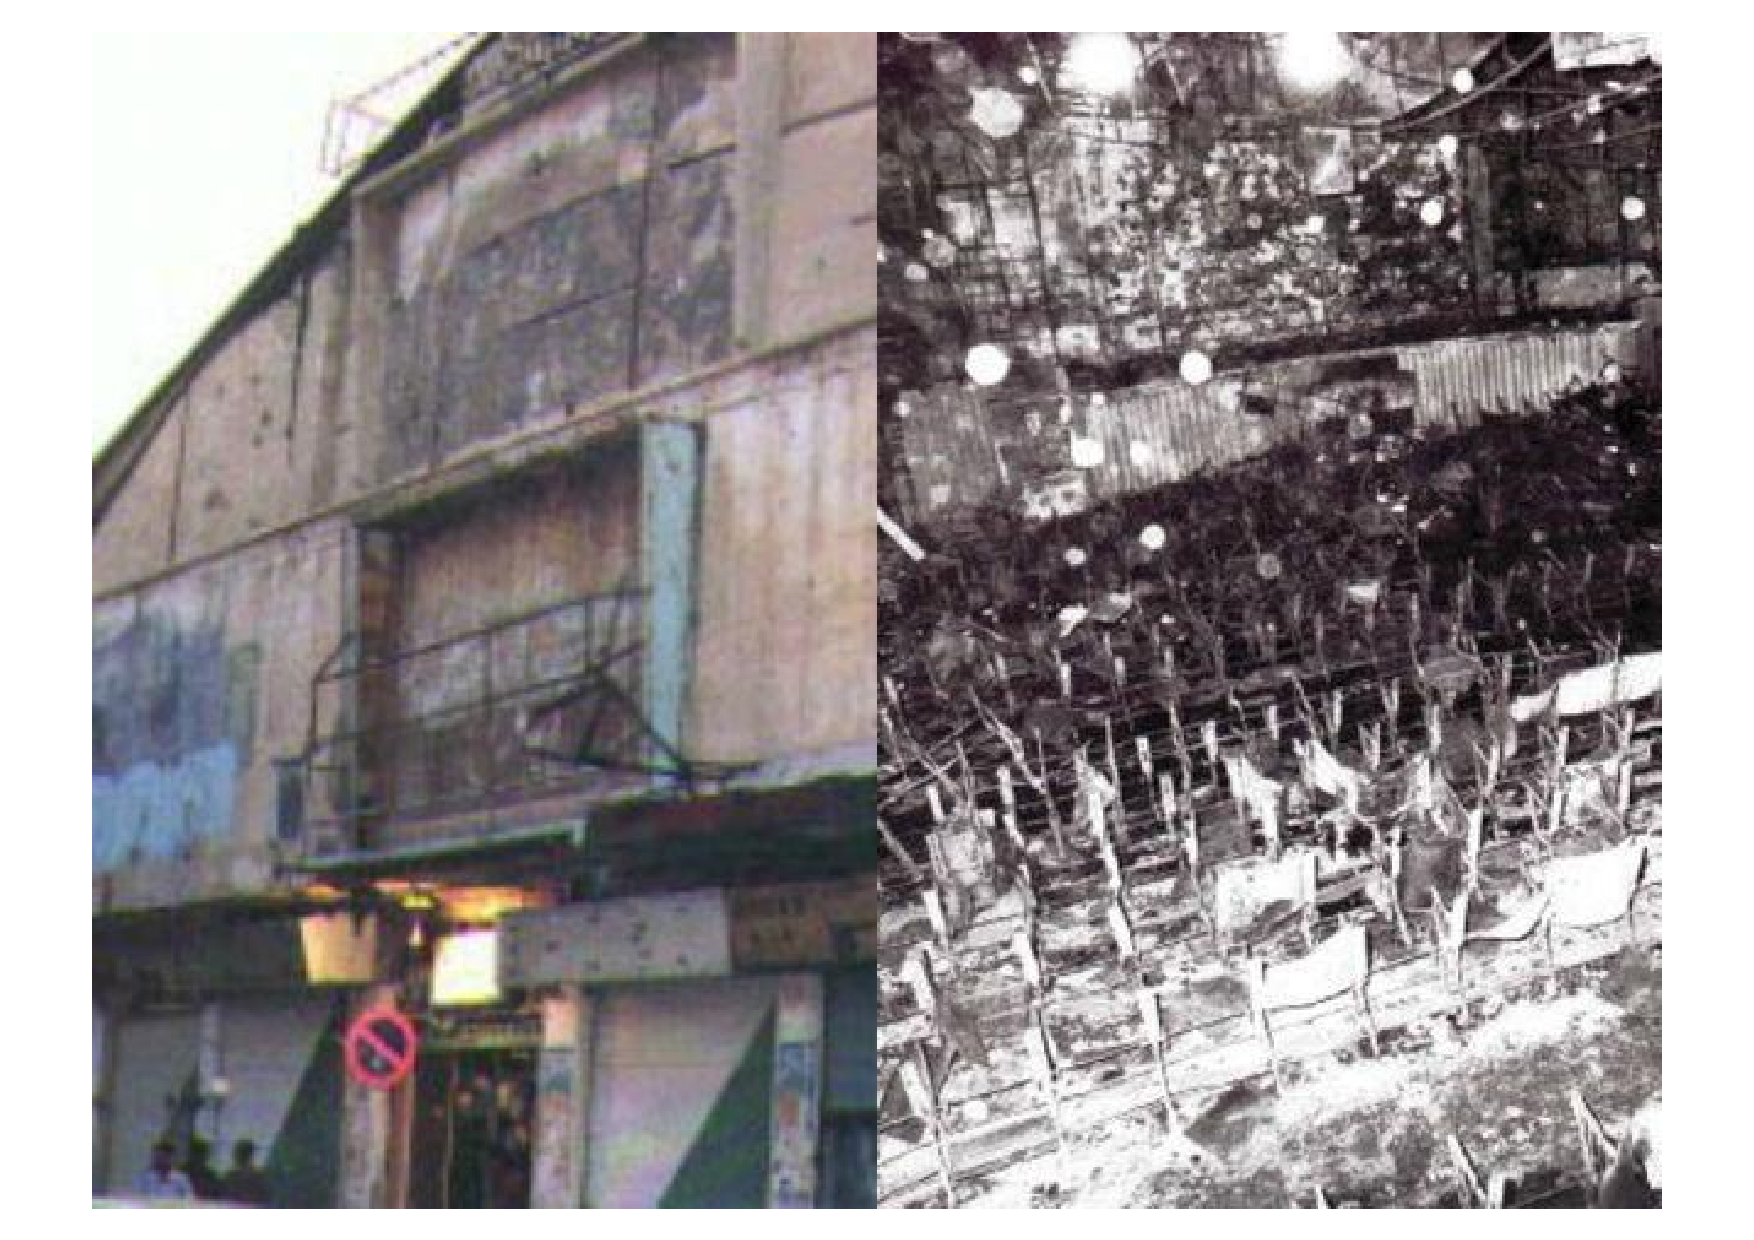
\includegraphics[height=110pt]{imagem1.pdf}
 \caption{Incêndio no cinema Rex.}
 \end{figure}

% Imagem 2 %
 \begin{figure}[h]
 \center
 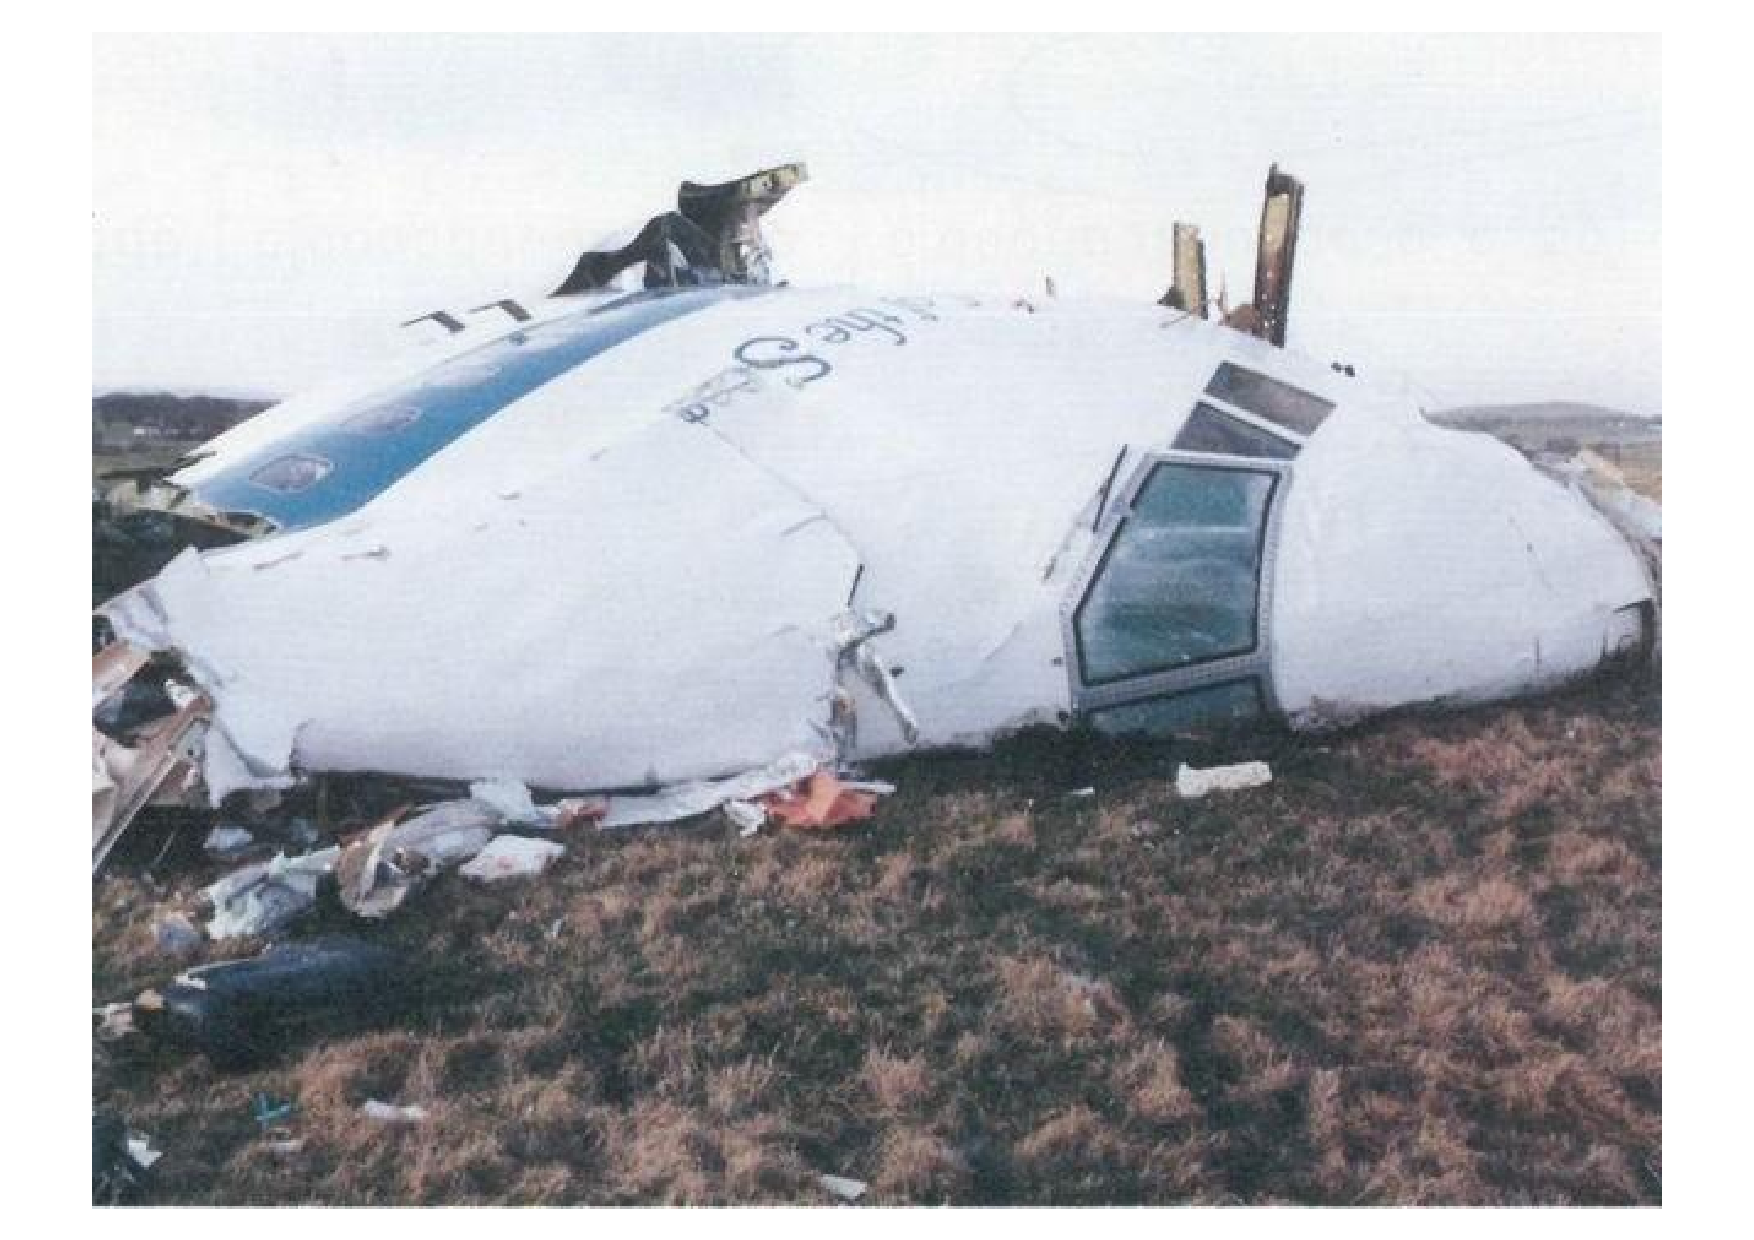
\includegraphics[height=110pt]{imagem2.pdf}
 \caption{Atentado de Lockerbie.}
 \end{figure}

% Imagem 3 %
 \begin{figure}[h]
 \center
 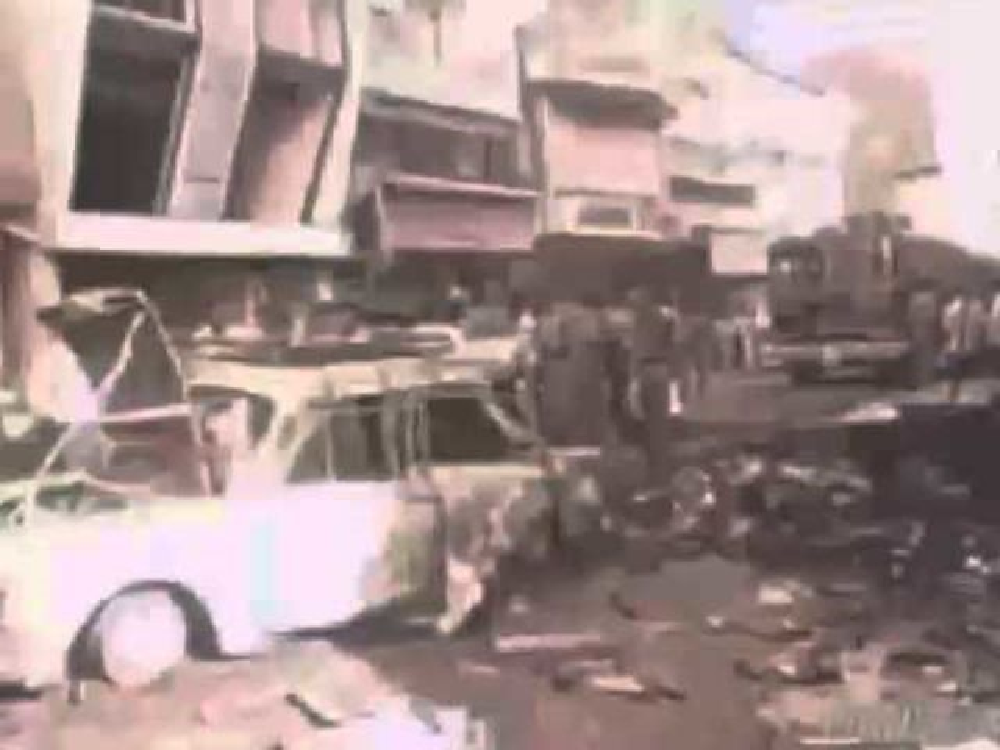
\includegraphics[height=110pt]{imagem3.pdf}
 \caption{Atentados de Bombaim.}
 \end{figure}

% Imagem 4 %
\begin{figure}[h]
 \center
 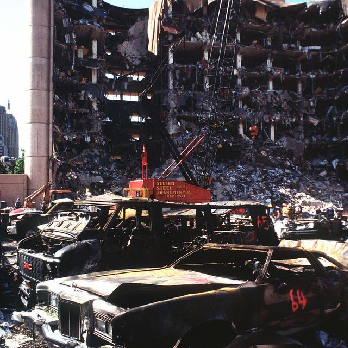
\includegraphics[height=110pt]{imagem4.pdf}
 \caption{Atentado de Oklahoma.}
 \end{figure}

% Imagem 5 %
\begin{figure}[h]
 \center
 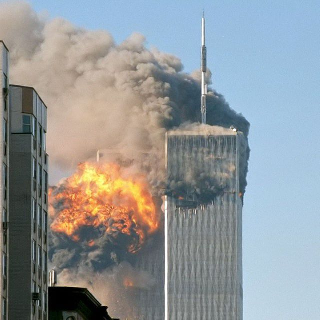
\includegraphics[height=110pt]{imagem5.pdf}
 \caption{Ataque ao World Trade Center, Torres Gémeas e Pentágono.}
 \end{figure}

% Imagem 6 %
\begin{figure}[h]
 \center
 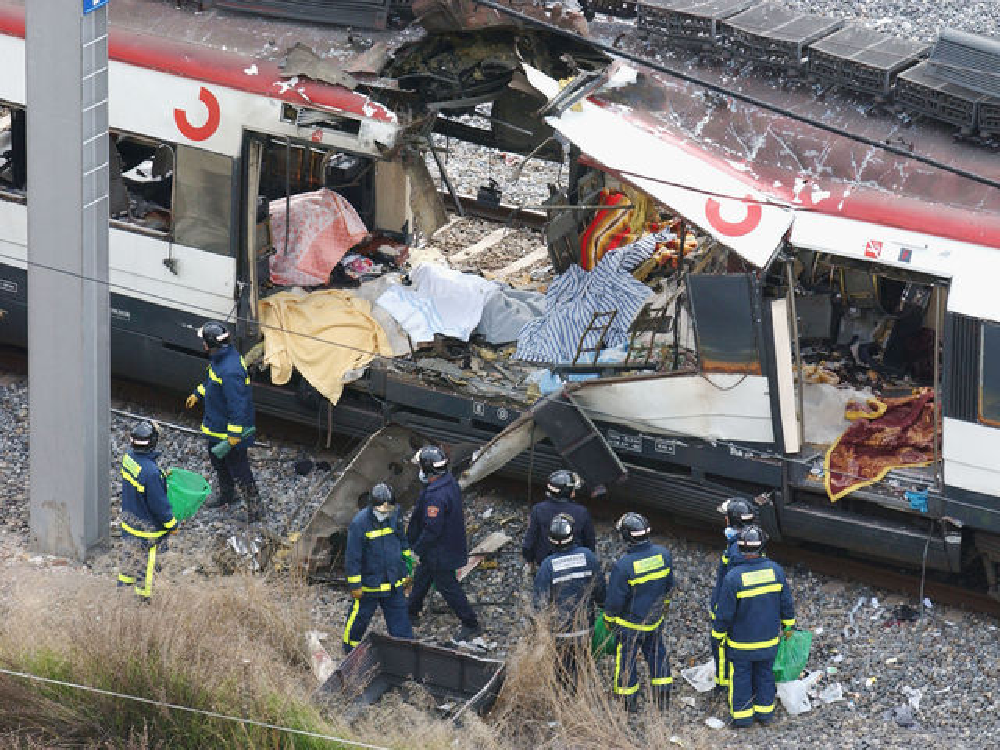
\includegraphics[height=110pt]{imagem6.pdf}
 \caption{Atentado de Madrid.}
 \end{figure}

% Imagem 7 %
\begin{figure}[h]
 \center
 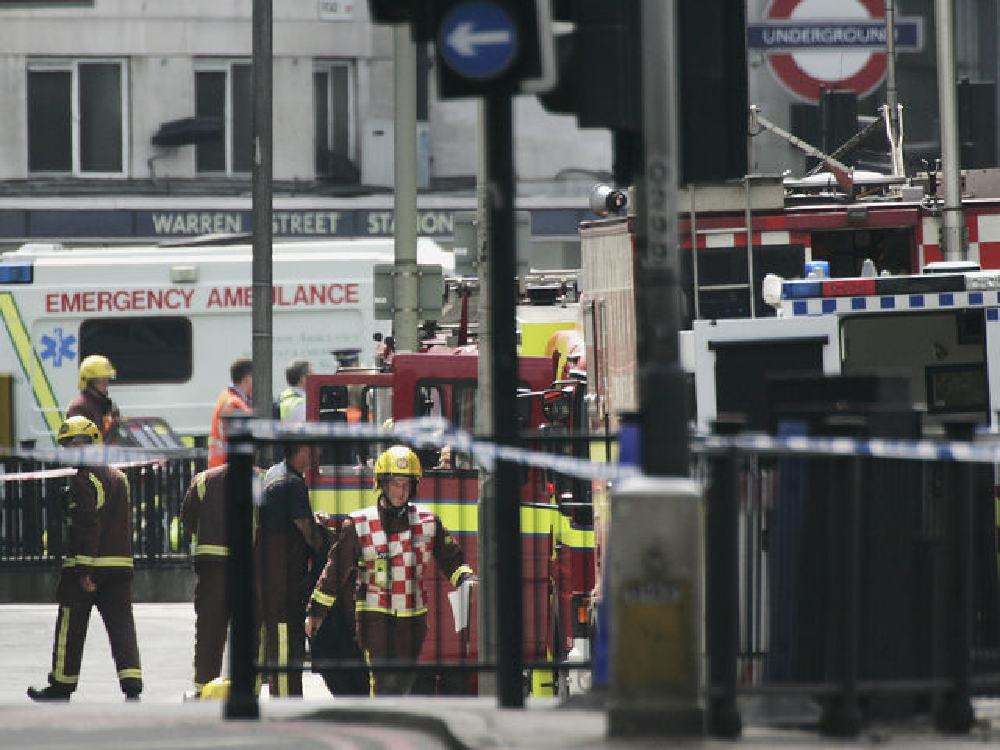
\includegraphics[height=110pt]{imagem7.pdf}
 \caption{Atendado ao metro de Londres.}
 \end{figure}

% Imagem 8 %
\begin{figure}[h]
 \center
 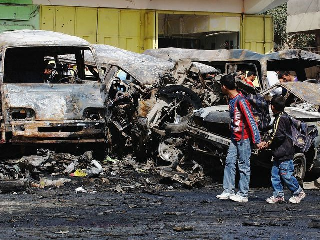
\includegraphics[height=110pt]{imagem8.pdf}
 \caption{Ataques de Sadr.}
 \end{figure}
 
% Imagem 9 %
\begin{figure}[h]
 \center
 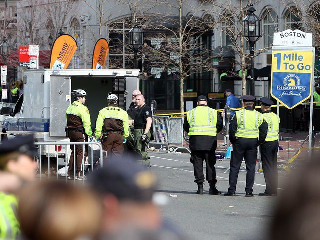
\includegraphics[height=110pt]{imagem9.pdf}
 \caption{Maratona de Boston.}
 \end{figure}
 
% Imagem 10 %
\begin{figure}[h]
 \center
 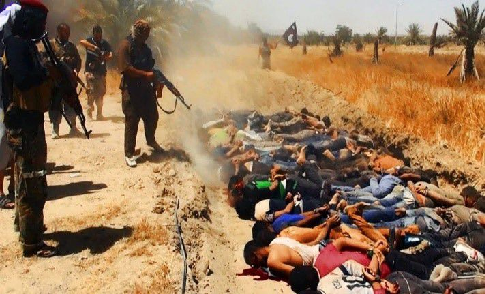
\includegraphics[height=110pt]{imagem10.pdf}
 \caption{Massacre de Sinjar.}
 \end{figure}


% Capítulo 11 - Definição de Ciberterrorismo %
\chapter{Definição de Ciberterrorismo}
\label{chap.Definição de Ciberterrorismo}
\paragraph{} As noções de ciberterrorismo podem datar desde o início de 1990, quando o uso da Internet despoletou e surgiram vários estudos acerca dos potenciais riscos apresentados pela grande afluência de informação facilmente alcançável.\par 
Segundo Dorothy Denning,
\begin {quotation}
"O ciberterrorismo é a convergência entre o ciberespaço e o terrorismo. Este refere-se a ataques ilegais e ameaças de ataques a computadores e informações armazenadas com o intuito de intimidar o governo e/ou as pessoas envolvidas devido a objetivos políticos ou sociais. No entanto, para se qualificar como ciberterrorismo, o ataque deve resultar em violência contra pessoas ou propriedades ou, pelo menos, causar grande impacto para gerar medo."
\end {quotation}
\par
O conceito de ciberterrorismo está inserido no conceito de terrorismo, já que se trataria de um ato de terrorismo praticado por meio cibernético ou através das novas tecnologias. O uso da Internet e de meios eletrónicos para fins terroristas, o ataque a infraestruturas eletrónicas também elas ligadas a Internet são ciberterrorismo.\par
Este tipo de terrorismo tem vindo a aumentar cada vez mais, sendo motivo de crescente preocupação a nível mundial pelas suas possíveis consequências económicas e danos que podem provocar ao normal funcionamento de um país.\par
O ciberterrorismo é uma opção atrativa para os terroristas modernos por diversas razões:
\begin{itemize}
  \item é mais barato do que os métodos tradicionais de terrorismo;
  \item é mais anónimo;
  \item a variedade e número de alvos é maior;
  \item pode ser conduzido remotamente;
  \item tem a capacidade de afetar diretamente um maior número de pessoas.
\end{itemize}
\par
Quando se fala em ataque cibernético, deparamo-nos com dois conceitos: a \textit{ciberguerra} e o \textit{ciberterrorismo}. \par
A \underline{ciberguerra} é uma guerra, entendida como o confronto entre dois ou mais grupos distintos de indivíduos mais ou menos organizados, realizada através de computadores e da internet.\par
O que difere uma guerra virtual de uma guerra física é meramente a substituição dos soldados armados frente-a-frente com o inimigo, pelos soldados munidos de tecnologia, sendo o campo de batalha,  virtual.
Os \underline{atos do ciberterrorismo} são fundados em motivações políticas, ideológicas ou sociais e em operações de \textit{hacking}. Tem como objetivo, causar prejuízos severos, desde perda de vidas humanas, prejuízos económicos, ataques ou ameaças contra sistemas informáticos, redes e a respetiva informação neles armazenada, de forma a intimidar ou coagir um governo. Pretende incutir medo e terror.\par
A globalização agravou em muito os problemas do ciberterrorismo e, para combater e precaver os atos de ciberterrorismo                                                                                                                                                                                                                                                                                existe cada vez mais, um maior intercâmbio entre os países.


% Capítulo 12 - Formas de Ciberterrorismo %
\chapter{Formas de Ciberterrorismo}
\label{chap.Formas de Ciberterrorismo}
\begin{tabular}{ | p{3.5cm} |p{8cm}| }
\hline
\center
\textbf{Vírus Informáticos} & São programas que, após serem executados, duplicam-se e infetam outros ficheiros dos computadores propagando-se. Contudo, nem todos são destrutivos. \\ \hline
\center
\textbf{Worms} & Propagam-se através das redes informáticas atacando \textit{hosts} vulneráveis, infetando-os e fazendo uso disso para se propagarem para outros alvos vulneráveis. Apagam ficheiros do computador anfitrião e enviam para os criminosos informação sensível e confidencial dos computadores infetados. \\ \hline
\center
\textbf{Trojans} & Não se reproduzem usando outros ficheiros e não se propagam eles próprios, tendo de ser transferidos e executados deliberadamente pelos utilizadores dos sistemas informáticos pois tendem a parecer ficheiros inofensivos, mas na realidade apagam ficheiros, alteram as configurações do sistema operativo e abrem \textit{backdoors} para que os criminosos entrem nos computadores infetados de forma a obter controlo sobre eles, podendo roubar/destruir/adulterar informação confidencial. \\ \hline
\center
\textbf{Spyware} & Não se reproduzem através de outros ficheiros, mas violam a privacidade das organizações, empresas e indivíduos ao enviar informação para os criminosos. Também, normalmente alteram a configuração dos sistemas. Exemplos: entrega de publicidade por correio eletrónico e pop-ups.\\ \hline
\end{tabular}

\begin{tabular}{ | p{3.5cm} |p{8cm}| }
\hline
\center
\textbf{SPAM} & Envio de mensagens publicitárias não solicitadas em grande escala, normalmente via correio eletrónico, contendo às vezes hiperligações para sítios eletrónicos que contém vírus.\\ \hline
\center
\textbf{Phishing} & Tentativa de conseguir dados pessoais para depois serem usados para lesar os afetados. Inclui o furto de identidade, roubo de cartão de crédito, senhas de acesso a contas na Internet, entre outros. É alterado o design de sítios eletrónicos fazendo-os parecer de organizações legítimas, onde os indivíduos fornecem seus dados pessoais que são depois roubados e usados para proveito próprio ou para financiar atividades ilícitas.\\ \hline
\end{tabular}


% Capítulo 13 - Níveis de Capacidade Ciberterrorista %
\chapter{Níveis de Capacidade Ciberterrorista}
\label{chap.Níveis de Capacidade Ciberterrorista}
\paragraph{} O Centro de Estudos do Terrorismo e de Guerra Irregular, da Naval Postgraduate School, definiu três níveis de capacidade ciberterrorista:
\begin{itemize}
  \item Simples/ Não estruturado;
  \item Complexo/ Coordenado;
  \item Avançado/ Estruturado;
\end{itemize}
\par
O nível Simples/ Não Estruturado descreve a capacidade da organização para conduzir ações básicas de \textit{hacking} contra sistemas individuais, utilizando ferramentas desenvolvidas por terceiros. A organização possui um fraco nível de análise de alvos, comando e controlo e capacidade de aprendizagem.\par
O nível Complexo/ Coordenado carateriza a capacidade da organização para conduzir ataques mais sofisticados contra múltiplos sistemas ou redes e, possivelmente, modificar ou criar ferramentas básicas de \textit{hacking}. A organização possui uma análise de alvos elementar, comando e controlo e capacidade de aprendizagem.\par 
O nível Avançado/ Estruturado materializa a possibilidade da organização poder conduzir ataques coordenados, suscetíveis de provocar uma disrupção massiva contra defesas integradas e heterogéneas (incluindo criptografia). A organização reúne as competências necessárias para criar sofisticadas ferramentas de \textit{hacking}, revelando uma eficiente análise de alvos, comando e controlo e capacidade de aprendizagem.


% Capítulo 14 - Exemplos de Atos de Ciberterrorismo %
\chapter{Exemplos de Atos de Ciberterrorismo}
\label{chap.Exemplos de Atos de Ciberterrorismo}

\begin{itemize}
   \item Em 2005 e 2007, no Brasil, houve várias zonas do país que ficaram sem luz, causadas por ataques de \textit{hackers}.
   \item Em 1997, um jovem \textit{hacker} desativou a torre de controlo de tráfego aéreo no aeroporto em Worcester, Massachusetts, que afetou o serviço aéreo.
   \item Em 2001, dois estudantes de pós-graduação conseguiram aceder ao sistema bancário usado para transações na Internet do departamento do banco do tesouro.
\end{itemize}


% Capítulo  15 - Conclusões %
\chapter{Conclusões}
\label{chap.conclusao}
\paragraph{} Enquanto cidadãos do mundo, vivemos desafiados a procurar a paz, bem-estar e respeito ao próximo todos os dias. No entanto, nem todos são capazes de manter uma mente aberta capaz de tolerar as diferenças – sejam elas sociais, económicas, religiosas, culturais, etc. Os atos terroristas provêm dos indivíduos que não são capazes de aceitar estas diferenças, tendo uma atitude fundamentalista e intolerante, servindo-se de ações extremistas e doentias para vincular e afirmar as suas ideologias e opiniões. São estas ações que desestabilizam uma sociedade, deixando-a fragilizada e escrava do medo.\par
Mas mais importante do que não deixar que o medo se apodere dos indivíduos, é não permitir que esse medo os leve a abdicar dos direitos da Humanidade, que tantos séculos levaram a ser conquistados. Isto porque, os atos terroristas violam alguns dos artigos presentes na Declaração Universal dos Direitos Humanos, tais como:
\begin {quotation}
"Artigo I: Todas as pessoas nascem livres e iguais em dignidade e direitos. São dotadas de razão e consciência e devem agir em relação umas às outras com espírito de fraternidade."
\end {quotation}

\begin {quotation}
"Artigo III: Toda pessoa tem direito à vida, à liberdade e à segurança pessoal."
\end {quotation}
   		 
\begin {quotation}
"Artigo V: Ninguém será submetido à tortura, nem a tratamento ou castigo cruel, desumano ou degradante."
\end {quotation}	 
   		
\begin {quotation}
"Artigo XXII: Toda pessoa, como membro da sociedade, tem direito à segurança social e à realização, pelo esforço nacional, pela cooperação internacional e de acordo com a organização e recursos de cada Estado, dos direitos económicos, sociais e culturais indispensáveis à sua dignidade e ao livre desenvolvimento da sua personalidade."
\end {quotation}
 
E se, através dos métodos tradicionais o terrorismo já assombra toda uma sociedade, com o despertar da era tecnológica e da sua dependência, a probabilidade de sofrer um ato terrorista aumenta significativamente. Isto porque, apesar de os ciberterroristas não serem motivados pelos mesmos objetivos que os terroristas convencionais, estes têm demonstrado uma facilidade absurda em aceder a informação sensível não só de indivíduos como também de empresas, provocando uma sensação de insegurança cada vez maior. 



% Contribuições dos autores %
\chapter*{Contribuições dos autores}

\paragraph{} Na distribuição do trabalho não sobrecarregar nenhum dos autores do documento. Tentámos fazer uma distribuição o mais justa possível. Assim, a MP focou-se no resumo, nos capítulos 3,8 e conclusão, a RA focou-se no introdução, capítulo 4, 5, 8, 14 e em conjunto pesquisámos material para os capítulos 2, 6, 7, 9, 10, 11, 13.
Depois do exposto, pode-se dizer que a percentagem de contribuição de cada autor foi de 50 por cento.

%%%%%%%%%%%%%%%%%%%%%%%%%%%%%%%%%
\chapter*{Acrónimos}

\begin{acronym}
\acro {UA}[\textit{UA}] {Universidade de Aveiro}
\end{acronym}


\begin{acronym}
\acro {URSS}[\textit{URSS}] {União das Repúblicas Socialistas Soviéticas}
\end{acronym}


\begin{acronym}
\acro {PPTS}[\textit{PPTS}] {Perturbação Pós-Stress Traumático}
\end{acronym}


\begin{acronym}
\acro {ETA}[\textit{ETA}] {Euskadi Ta Askatasuna}
\end{acronym}


\begin{acronym}
\acro {IRA}[\textit{IRA}] {Irish Republican Army}
\end{acronym}


\begin{acronym}
\acro {EUA}[\textit{EUA}] {United States of America}
\end{acronym}


\begin{acronym}
\acro {PNV}[\textit{PNV}] {Partido Nacionalista Basco}
\end{acronym}


\begin{acronym}
\acro {ISIS}[\textit{ISIS}] {Islamic State of Iraq and Syria}
\end{acronym}


\begin{acronym}
\acro {FARC}[\textit{FARC}] {Forças Armadas Revolucionárias da Colômbia}
\end{acronym}


% Bibliografia %
\printbibliography
\chapter*{Bibliografia}

\begin{itemize}
 \item  \url {Junior, A. G. (2013).  Obtido de https://www.infoescola.com/historia/exercito-republicano-irlandes-ira/}
 \item  \url {(s.d.). https://pt.wikipedia.org/wiki/Al-Qaeda}
 \item  \url {Presse, F. (s.d.). Obtido de http://www1.folha.uol.com.br/folha/mundo/ult94u103629.shtml}
 \item  \url {(s.d.). http://www.elmundo.es/eta/historia/}
 \item  \url {(s.d.). http://terroremescala.blogs.sapo.pt/3553.html}
 \item  \url {Sofia Rosa, C. P., & Franco, H. (s.d.). 2016. Obtido de http://multimedia.expresso.pt/ataques terroristas mundo/}
 \item  \url {(s.d.). https://canalcienciascriminais.jusbrasil.com.br/artigos/355635019/mas-afinal-o-que-e-ciberterrorismo}
 \item  \url {(s.d.). http://brasilescola.uol.com.br/geografia/grupos-terroristas-mundo.htm}
 \item  \url {(s.d.). https://www.usip.org/sites/default/files/sr119.pdf}
 \item  \url {(s.d.). http://www.itpro.co.uk/security/29726/what-is-cyber-terrorism}
 \item  \url {(s.d.). https://worldview.stratfor.com/weekly/coming-age-cyberterrorism}
 \item  \url {(s.d.). https://www.techopedia.com/definition/6712/cyberterrorism}
 \item  \url {(s.d.). https://www.steptoe.com/publications/231a.pdf}
 \item  \url {(s.d.). http://www.wussu.com/current/levine.htm}
 \item  \url {(s.d.). http://www.terrorism-research.com/history/early.php}
 \item  \url {(s.d.). http://forensic-psychology.net/2016/08/15/is-terrorism-successful/}
\end {itemize}

\end{document}